\section{Solving constrained problems}\label{constrained}
We will now consider the problem \ref{eq:basic problem}, where the set of admissible solutions is given by \ref{eq:admissible solution}. In this section, we describe how to generally solve this problem by converting it into a sequence of unconstrained optimization problems. There exist several other methods for solving constrained problems, but here we will focus on the penalty and the barrier methods.

\subsection{Penalty methods}\label{penalty method}
As mentioned earlier, penalty methods convert constrained optimization problems into unconstrained ones. The fundamental principle of penalty methods is to incorporate the conditions that define the set of admissible solutions by adding a penalty term to the objective function, which reflects the degree of violation of those conditions \cite{Bert}. The penalty function is defined as a continuous scalar function on $ \mathbb{R}^n $ that satisfies

\begin{align}
	\begin{split}
		p(\vec{x}) &= 0, \ \ \forall \vec{x} \in \mathbf{X},\\[6pt]
		p(\vec{x}) &> 0, \ \ \text { otherwise. }
	\end{split}
\end{align}
A typical choice for the penalty function is, e.g.,
\begin{equation}\label{eq:penalty function}
	p (\vec{x}) = \sum_{j=1}^{m} \left( \, \max  \left\{ \, g_j \, (\vec{x}), 0 \, \right\} \, \right)^2 + \sum_{j=1}^{q} h_j (\vec{x})^2.
\end{equation}
Using the penalty function $ p $, we construct the modified objective function
\begin{equation}\label{eq:cost function with penalty}
	\phi (\vec{x}, r) = f (\vec{x}) + r p(\vec{x}),
\end{equation}
where $ r > 0 $ is called the penalty coefficient \cite{Bert}. From the definition of the penalty function, it can be seen that the values of the modified objective function $ \phi (\vec{x}, r)$ differ from the original function $ f $ only for such $ \vec{x} $ that violate the specified condition.

To solve the constrained problem, we iteratively construct a new term in an increasing sequence of penalty coefficients $ r_1, r_2, \dots$, for which we solve the unconstrained optimization problem for the modified function $ \phi (\vec{x}, r_k)$. The optimal solution $ \vec{x}_k $ of this unconstrained problem is then used as the starting point for the next iteration. This process is repeated until the condition $ r_k p(\vec{x}_k) < \varepsilon$ for some $ \varepsilon > 0$ is satisfied. When this condition is met, $ \vec{x}_k $ can be considered a sufficiently accurate approximation of the solution to the constrained problem. It should be noted that penalty methods allow searching for an optimal solution outside the set of admissible solutions during the iterations \cite{non-linear-textbook}, and thus are categorized as exterior point methods. A key assumption of penalty methods is that the domain of the problem satisfies $ \mathbf{D} = \mathbb{R}^n $.

The construction of the sequence of penalty parameters and the principle of the penalty method are illustrated in Figure~\ref{fig:penalty} on a trivial example of minimizing the function $ f(x) = 0.5x $ with the constraint $ g(x) = 4 - x \leq 0 $. The modified objective function in this case takes the form
\begin{equation}
	\phi (x, r) = 0.5x + r \left(\max  \left\{ \,  4-x, 0 \right\}\right)^2.
\end{equation}
\begin{figure}[H]
	\vspace{-2.25cm}
	\centering
	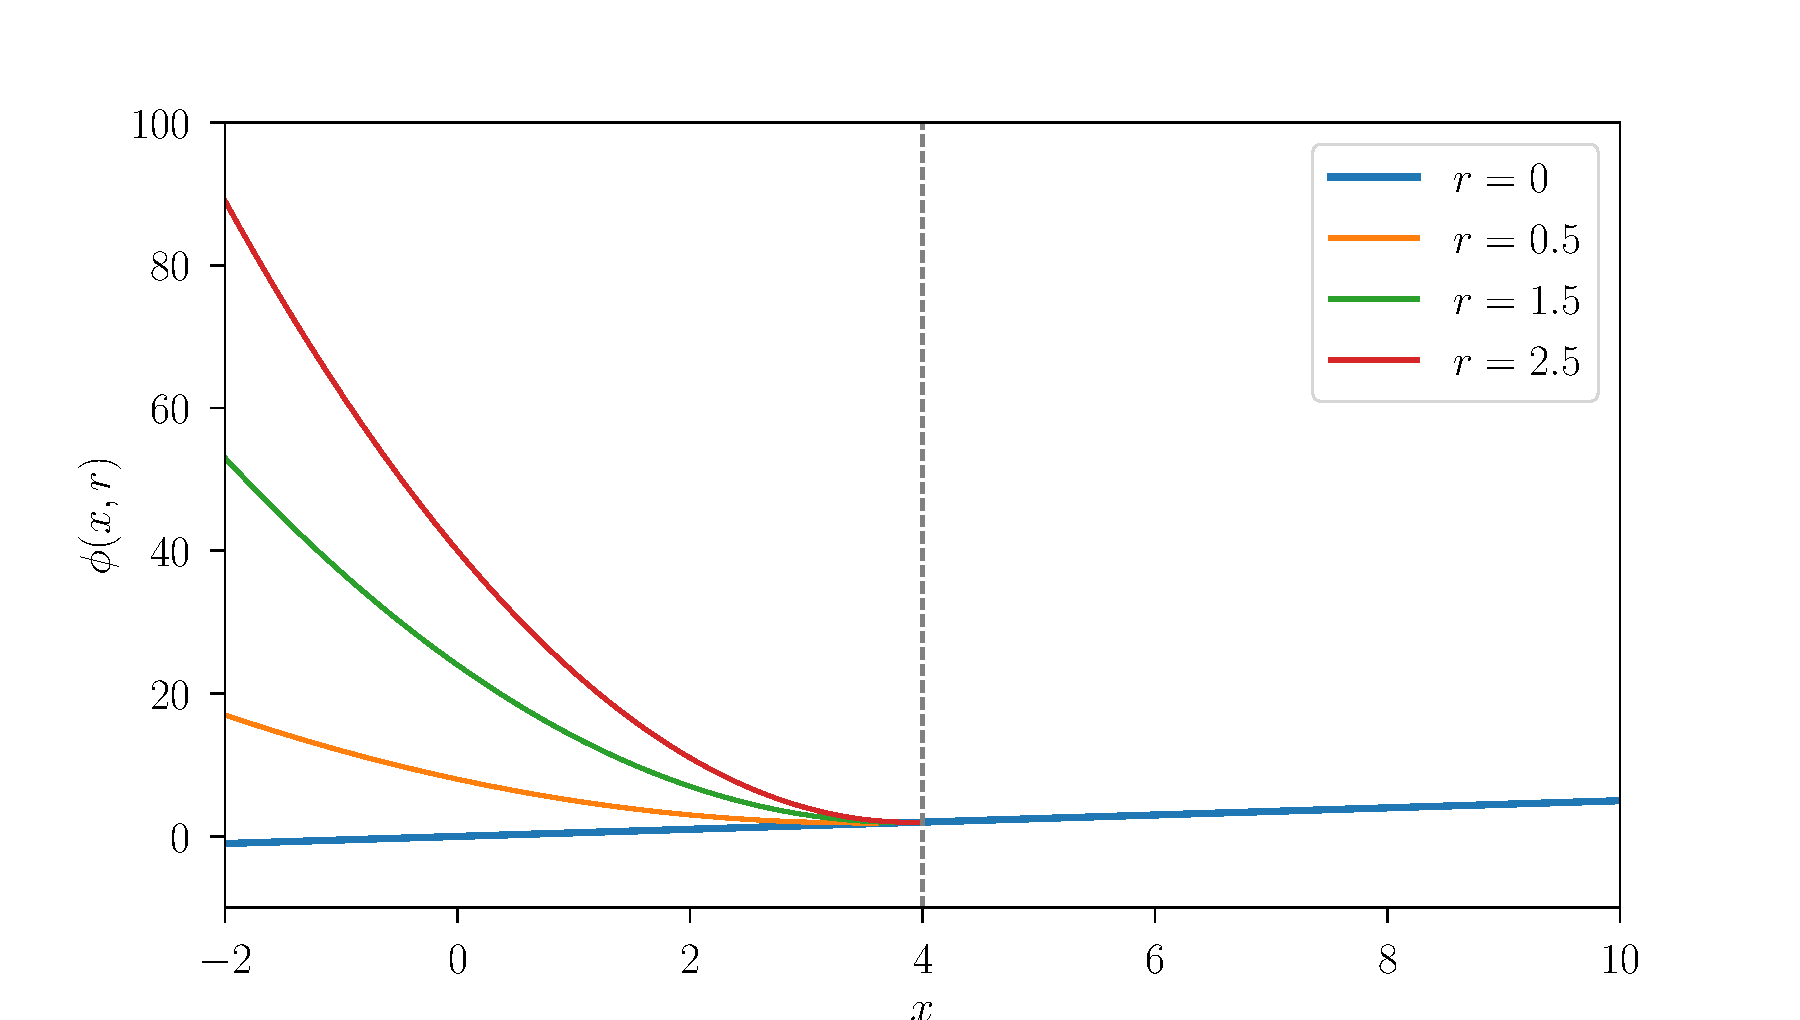
\includegraphics[width=0.9\textwidth]{figures/penalty.pdf}
%	\vspace{0.2cm}
	\caption{An illustration of the penalty method applied to minimizing the function $ f(x) = 0.5x $ with the constraint $ g(x) = 4 - x \leq 0 $. Different shapes of the modified objective function $ \phi (x, r) $ depending on the value of the penalty parameter $ r $ are distinguished by color. The condition defining the set of admissible solutions is indicated by the gray dashed line. The set of admissible solutions lies in the half-plane to the right of this gray dashed line.}
	\label{fig:penalty}
\end{figure}


\subsection{Barrier method}\label{barrier method}
The barrier method operates on a principle similar to that of the penalty method, but its main difference is that, during the iterative process of finding an optimal solution to a constrained problem, it ensures that the solution estimates always remain within the interior of the feasible set, which is defined as
\begin{equation}
	\mathbf{X}^{\mathrm{o}} = \left\{ \vec{x} \in \mathbf{D} \subseteq \mathbb{R}^n \ \middle| \ \vec{g}(\vec{x}) < \vec{0} \right\}.
\end{equation}
Methods that satisfy this condition are generally referred to as interior-point methods \cite{non-linear-textbook}.

As with penalty methods, we account for the conditions defining the feasible set by adding a new term to the objective function, which reflects the degree to which these conditions are violated. The barrier function $ B $ is a continuous scalar function on $ \mathbf{X}^{\mathrm{o}} $ that satisfies the condition
\begin{equation}
	(\exists j \in \{1,2,\dots,m\})(\lim\limits_{\substack{\vec{x} \to \vec{y} \\ \mathbf{X}^{\mathrm{o}}}} g_j (\vec{x}) = 0) \Rightarrow \lim\limits_{\substack{\vec{x} \to \vec{y} \\ \mathbf{X}^{\mathrm{o}}}} B (\vec{x}) = + \infty.
\end{equation}
A typical choice for the barrier function is the logarithmic barrier function
\begin{equation}\label{eq:log barrier function}
	B (\vec{x}) = -\sum_{j=1}^{m} \ln \left( - g_j (\vec{x}) \right),
\end{equation}
or the reciprocal barrier function
\begin{equation}\label{eq:reciprocal barrier function}
	B (\vec{x}) = -\sum_{j=1}^{m} \frac{1}{g_j (\vec{x})}.
\end{equation}
Using the barrier function $ B $, we construct the modified objective function
\begin{equation}\label{eq:cost function with barrier}
	\phi (\vec{x}, r) = f (\vec{x}) + r B(\vec{x}),
\end{equation}
where $ r > 0 $ \cite{non-linear-textbook}.

To solve the constrained problem using the barrier method, at each iteration we construct a new term in a strictly decreasing sequence of positive parameters $ r_1, r_2, \dots$, for which we solve the unconstrained optimization problem for the modified function $ \phi (\vec{x}, r_k)$. The vector $ \vec{x}_k  = \operatorname*{argmin}_{\vec{x} \in \mathbf{X}^\mathrm{o}} (f(\vec{x}) + r_k B(\vec{x})) $, obtained by optimizing the unconstrained problem, is used as the starting point for the next iteration. This process is repeated until the condition $ r_k < \varepsilon$ for some $ \varepsilon > 0$ is satisfied, at which point $ \vec{x}_k $ is considered a sufficient approximation to the solution of the constrained problem \cite{non-linear-textbook}.

The construction of the parameter sequence $ (r_k)_{k \in \mathbb{N}} $ and the principle of the barrier method are illustrated in Figure~\ref{fig:barrier} using the example of minimizing the function $ f(x) = 0.5x $ with the constraint $ g(x) = 4 - x \leq 0 $ and the choice of the reciprocal barrier function. The modified objective function in this case is
\begin{equation}
	\phi (x, r) = 0.5x - \frac{r}{4-x}.
\end{equation}

\begin{figure}[H]
	\centering
	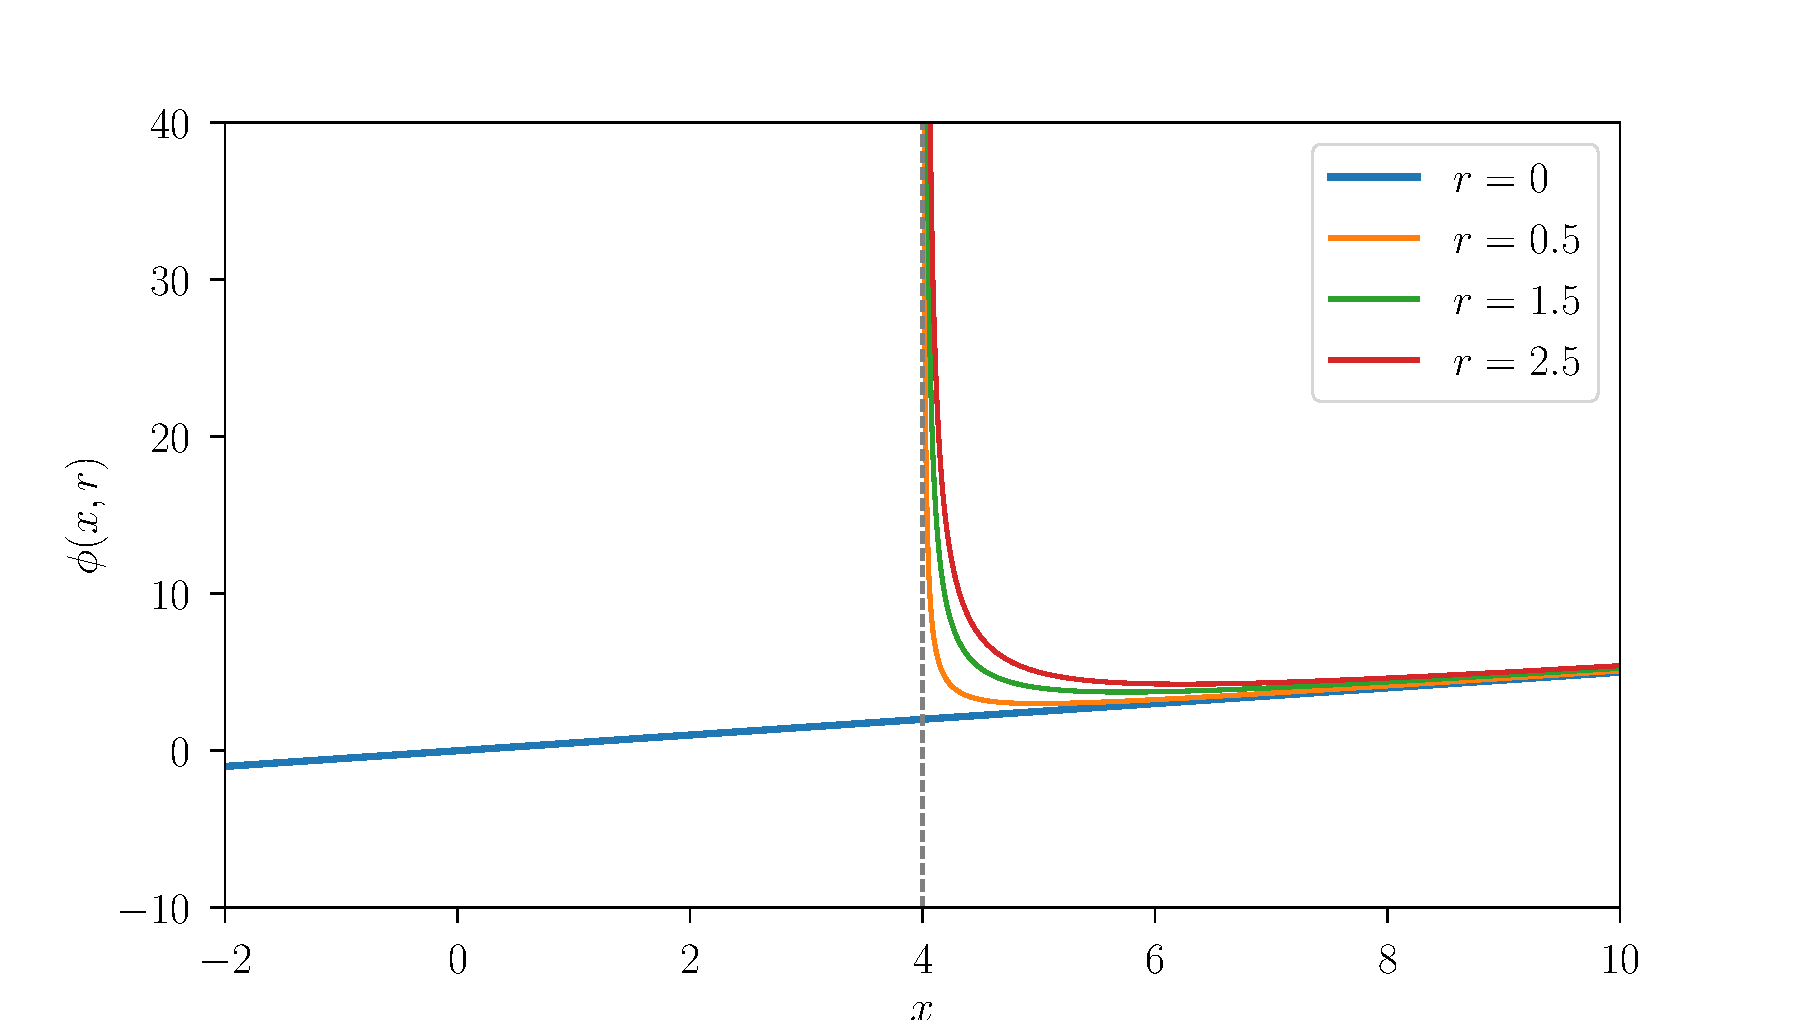
\includegraphics[width=0.9\textwidth]{figures/barrier.pdf}
	\caption{An illustration of the barrier method applied to minimizing the function $ f(x) = 0.5x $ with the constraint $ g(x) = 4 - x \leq 0 $. Different shapes of the modified objective function $ \phi (x, r) $ depending on the value of the barrier parameter $ r $ are distinguished by color. The condition defining the set of feasible solutions is indicated by the gray dashed line. The set of feasible solutions lies in the half-plane to the right of this gray dashed line.}
	\label{fig:barrier}
\end{figure}

Finally, we define the specific choice of the barrier function $ B_{\infty} $ called the extreme barrier function \cite{BBO-textbook}. This extreme barrier function mirrors the asymptotic behavior of the aforementioned barrier functions and is given by
\begin{align}
	\begin{split}
		B_{\infty}(\vec{x}) &= 0, \ \ \forall \vec{x} \in \mathbf{X},\\[6pt]
		B_{\infty}(\vec{x}) &= +\infty, \ \ \text{otherwise.}
	\end{split}
\end{align}
The modified objective function (extreme barrier function) is then given by
\begin{align}\label{eq:extreme barrier}
	\begin{split}
		f_{\infty}(\vec{x}) &= f(\vec{x}) , \ \ \forall \vec{x} \in \mathbf{X},\\[6pt]
		f_{\infty}(\vec{x}) &= +\infty, \ \ \text{otherwise.}
	\end{split}
\end{align}